\begin{figure}[!p]
    \centering
    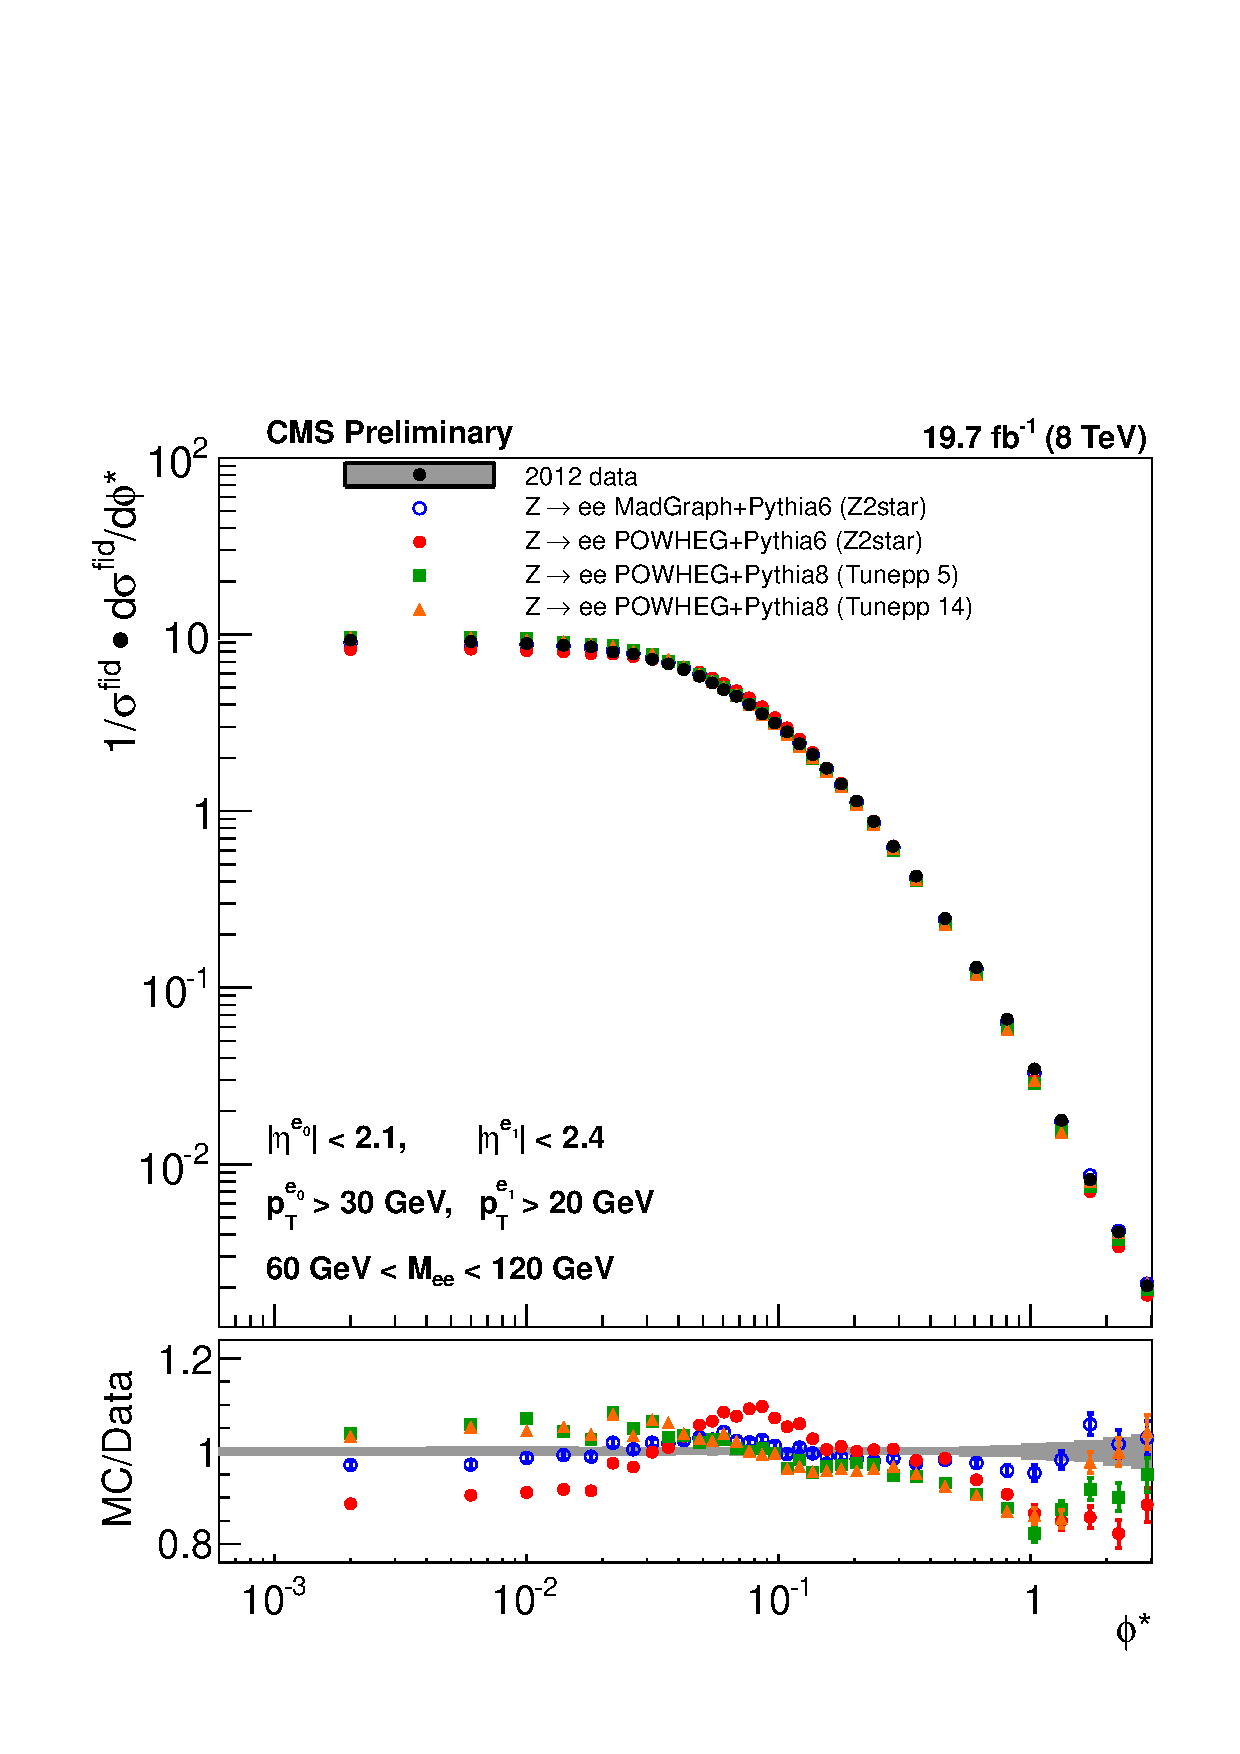
\includegraphics[width=\textwidth]{figures/ZShape_elec_PH_Norm_Dressed.pdf}
    \caption[
        The normalized differential cross section with respects to \phistar for
        \Ztoee events in our fiducial region from data and \MADGRAPH and
        \POWHEG unfolded with \POWHEG.
    ]{
        The normalized differential cross section with respects to \phistar for
        \Ztoee events in our fiducial region from data and \MADGRAPH and
        \POWHEG unfolded with \POWHEG. A close up of the lower plot is shown in
        \FIG~\ref{fig:results_ratio_norm_powheg}.
    }
    \label{fig:results_norm_powheg}
\end{figure}

\begin{figure}[!p]
    \centering
    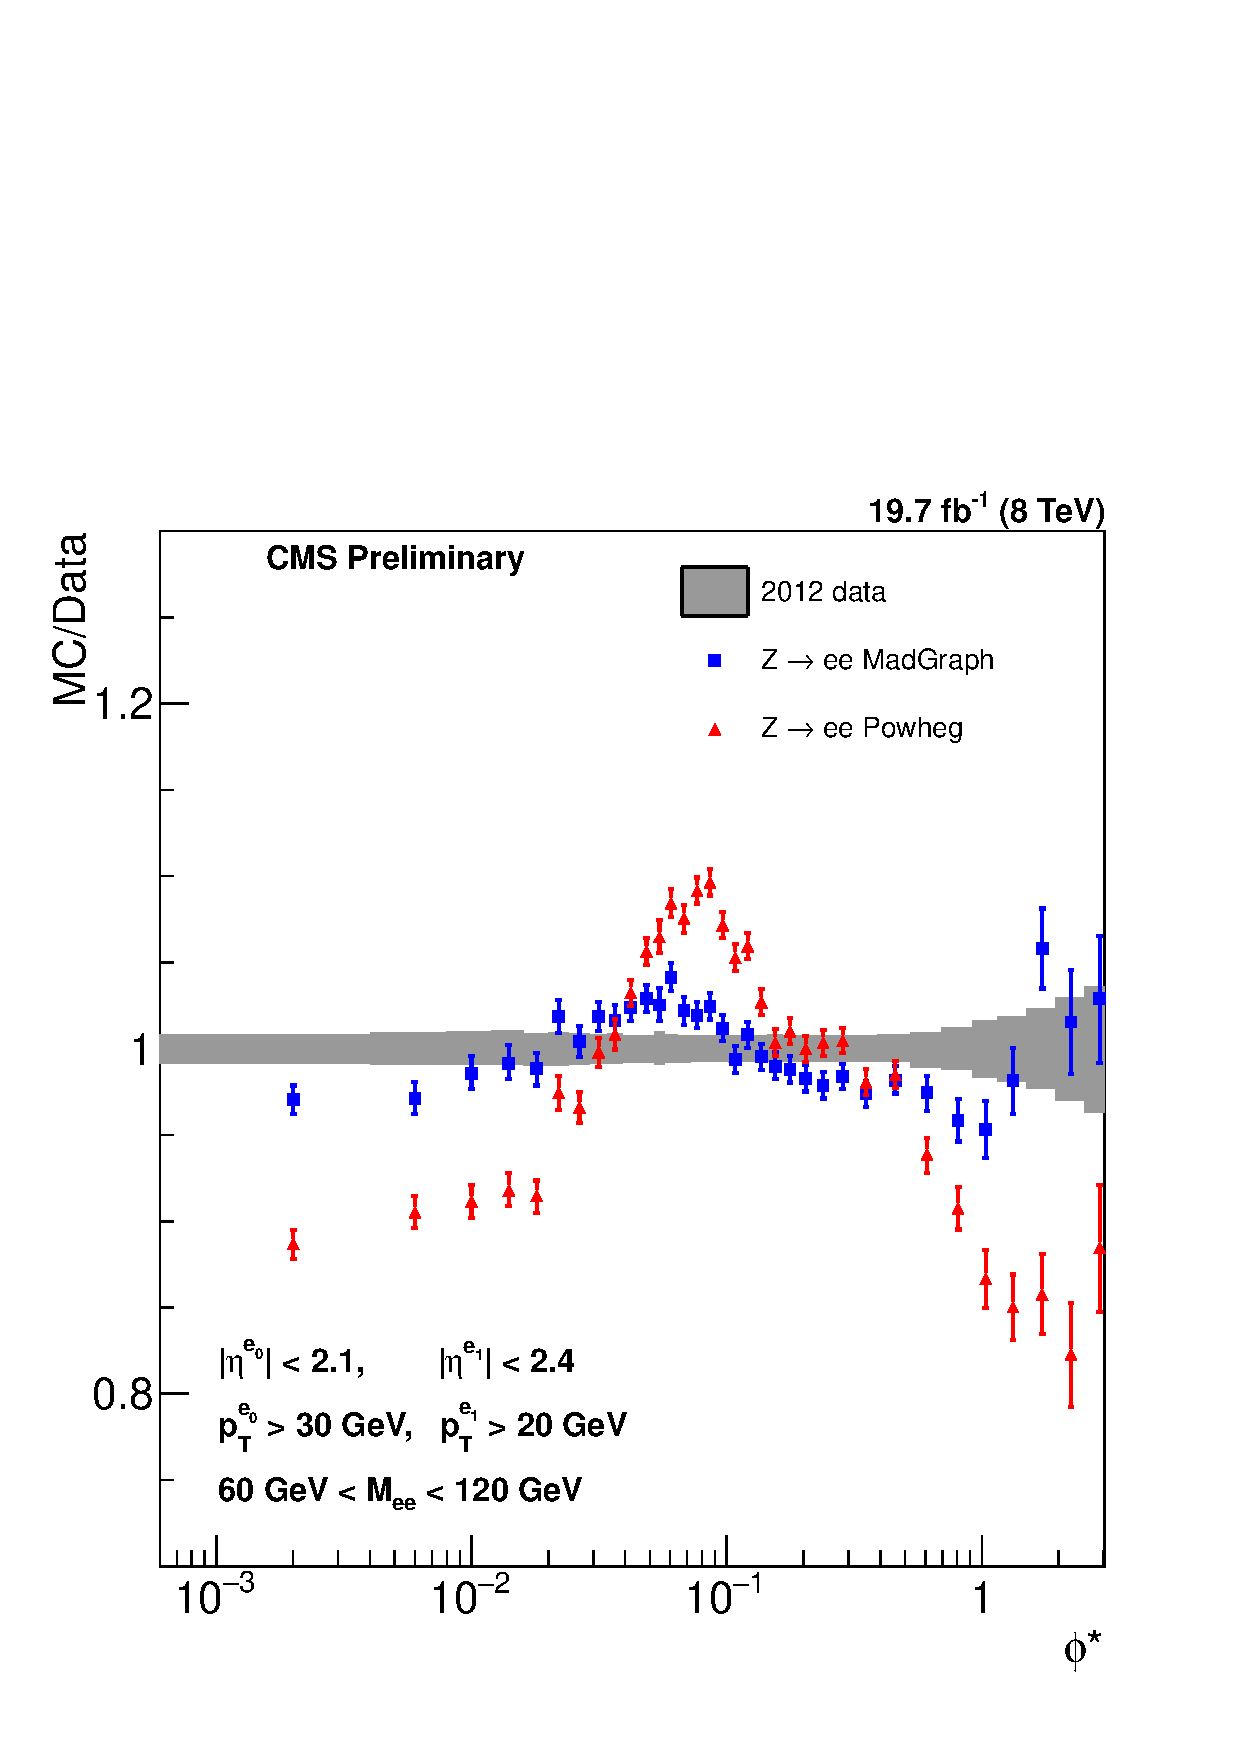
\includegraphics[width=\textwidth]{figures/ZShape_Ratioelec_PH_Norm_Dressed.pdf}
    \caption[
        Close up of the ratio plot from \FIG~\ref{fig:results_norm} for the
        normalized cross section measurement.
    ]{
        Close up of the ratio plot from \FIG~\ref{fig:results_norm} for the
        normalized cross section measurement unfolded with \POWHEG. The error
        band indicates the uncertainty in the data, while the square points
        show the ratio of \MADGRAPH over data, and the triangle points show the
        ratio of \POWHEG over data.
    }
    \label{fig:results_ratio_norm_powheg}
\end{figure}
